\documentclass[11pt]{article}

\usepackage{latexsym}
\usepackage{amsmath}
\usepackage{amssymb}
\usepackage{amsthm}
\usepackage{graphicx}
\usepackage{wrapfig}
\usepackage{pseudocode}
\usepackage{url}
\usepackage[backref, colorlinks=true, citecolor=red, urlcolor=blue, pdfauthor={Jyh-Ming Lien}]{hyperref}


\newcommand{\handout}[5]{
  \noindent
  \begin{center}
  \framebox{
    \vbox{
      \hbox to 5.78in { {\bf Advanced Algorithms} \hfill #2 }
      \vspace{4mm}
      \hbox to 5.78in { {\Large \hfill #5  \hfill} }
      \vspace{2mm}
      \hbox to 5.78in { {\em #3 \hfill #4} }
    }
  }
  \end{center}
  \vspace*{4mm}
}

\newcommand{\lecture}[4]{\handout{#1}{#2}{#3}{}{#1}}

\newtheorem{theorem}{Theorem}
\newtheorem{corollary}[theorem]{Corollary}
\newtheorem{lemma}[theorem]{Lemma}
\newtheorem{observation}[theorem]{Observation}
\newtheorem{proposition}[theorem]{Proposition}
\newtheorem{definition}[theorem]{Definition}
\newtheorem{claim}[theorem]{Claim}
\newtheorem{fact}[theorem]{Fact}
\newtheorem{assumption}[theorem]{Assumption}

% 1-inch margins, from fullpage.sty by H.Partl, Version 2, Dec. 15, 1988.
\topmargin 0pt
\advance \topmargin by -\headheight
\advance \topmargin by -\headsep
\textheight 8.9in
\oddsidemargin 0pt
\evensidemargin \oddsidemargin
\marginparwidth 0.5in
\textwidth 6.5in

\parindent 0in
\parskip 1.5ex
%\renewcommand{\baselinestretch}{1.25}

\begin{document}

\lecture{Program Assignment 1}{Fall 2015}{Prof.\ Jyh-Ming Lien}{---}

152cpg04 

Yunjoo Park

\href{mailto:yunjoopark12@gmail.com}{\it yunjoopark12@gmail.com}

git clone \href{https://github.com/yunjoopark/programmingAssignment1.git}{https://github.com/yunjoopark/programmingAssignment1.git}

In addition to the implementation of the algorithms, you also need to turn in a report in \LaTeX. 
Your report should include an overview of your implementation intuitions (e.g., how the circumsphere is computed, 
how the poles are found from qhull), all the example outputs, known bugs, and known limitations.


\section{Part 1: 3D Delaunay Triangulation}

\subsection{Problem definition and Analysis}
Let  $P := \{p_1,p_2,...,p_n\}$ be a set of points in the plane. In that, a \textit{triangulation} of $P$ is defined a maximal planar subdivision whose vertex set is $P$ and it denoted by $DT(P)$. When there are three points $p_i,p_j,p_k \in P$ are vertices in the same face of the $DT(P)$, the circle through $p_i,p_j,p_k$ contains no other points. This circle is called the circumcircle of the triangle defined by $(p_i,p_j,p_k)$. We can relatively easily compute the \textit{Delaunay Triangulate} by using convex hull( ``\href{http://www.qhull.org/}{qhull}").

\subsection{Platforms}
Languages: C

Platform: Microsoft visual Studio 2013

OS: Windows

\subsection{Examples of Inputs}

1. There are 11 test data.

2. Each data file has different values.

3. Each line has three value, $x, y, z$.

\subsection{Outputs}

\begin{figure}[h]

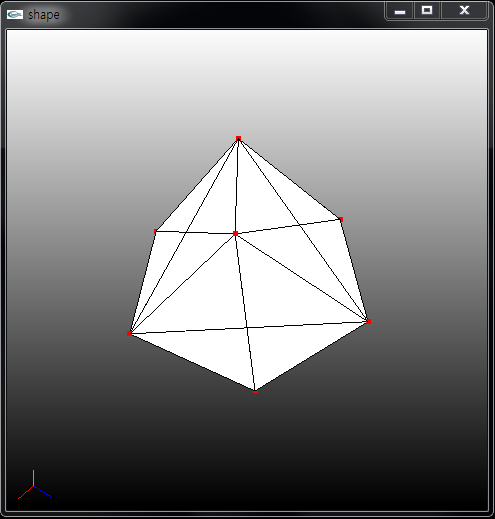
\includegraphics[width=.5\textwidth]{FIGS/icube-tetra}
\caption{An example of tetrahedra \textit{i.cube}}
\label{alg:alpha}
\end{figure}

\begin{figure}[h]
\centering
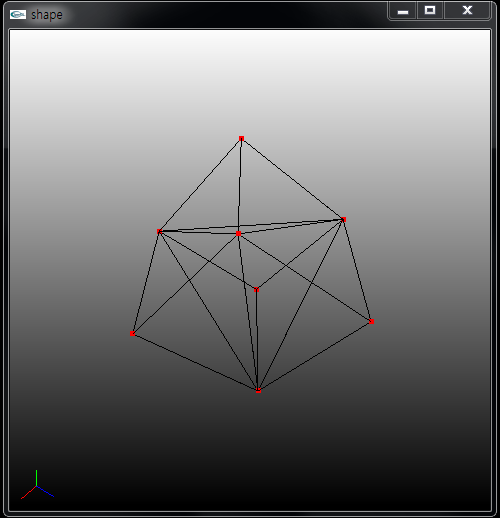
\includegraphics[width=.5\textwidth]{FIGS/icube-edges}
\caption{An example of edges \textit{i.cube}}
\label{alg:alpha}
\end{figure}




\section{Part 2: 3D $\alpha$-shape (30 pts)}


For a given value of $\alpha$, 
the $\alpha$-shape includes all the tetrahedra in the Delaunay triangulation which have an empty circumsphere with {\em squared radius} equal or smaller than $\alpha$.
Algorithm~\ref{alg:alphashape} sketches this idea. Examples of $\alpha$-shape is illustrated in Figure~\ref{alg:alpha}.
More detailed information about 3-d  $\alpha$-shape can be found in this 
\href{http://www.cgal.org/Manual/latest/doc_html/cgal_manual/Alpha_shapes_3/Chapter_main.html}{CGAL page} and in
the paper by Edelsbrunner and M\"{u}cke~\cite{em-tdas-94}.

{\small
	\begin{pseudocode}[shadowbox]{$\alpha$ shape}{P[1 \cdots n], \alpha}
	\label{alg:alphashape}
	\COMMENT{$P$ is a set $n$ points}\\
	D = \text{Delaunay triangulation of $P$} \\
	\FOREACH { \text{tetrahedron } t \in D} \DO
	\BEGIN
	\IF \text{the circumsphere of $t$ has squared radius larger than $\alpha$}  \DO
		\text{Remove } t
	\END
	\end{pseudocode}
}


\begin{figure}[h]
\centering
\includegraphics[width=.5\textwidth]{FIGS/alphashape}
\caption{An example of alpha shape with different values}
\label{alg:alpha}
\end{figure}




\subsection{What should  you do?}

Your goal is to use \href{http://www.qhull.org/}{\it qhull} to implement Algorithm~\ref{alg:alphashape}.
%The package qhull will be provided but if you like, you can try to download and compile to latest version of it. 
The output of your program should remain the same as it is now, therefore
the provided OpenGL interface can understand your output.




\section{Part 3: Crust Algorithm (40 pts)}

This part is due on Oct 22, 11:59pm, 2015.


%\begin{wrapfigure}{r}{0.5\textwidth}
%\vspace{-1cm}
\begin{figure}[ht]
\centering
\includegraphics[width=.5\textwidth]{FIGS/crust-alg}
\caption{3D crust algorithm}
\label{alg:crust-alg}
%\vspace{-1cm}
%\end{wrapfigure}
\end{figure}

The idea of Crust for surface reconstruction is proposed by Nina Amenta et al. \cite{abk-anvra-98} in 1998.
Briefly, the crust of a set of points is a set of edges (in 2d) or triangles (in 3d) whose circumcircles is empty of
(1) input points and (2) the medial axis.  A complete crust algorithm is shown in Fig.~\ref{alg:crust-alg}.


The main challenge of this part of assignment is to find the poles for each site. The poles
of site $s$ are the furthest vertices of $s$'s Voronoi cell; one on each side of the surface. 
An example of the poles is shown in Fig.~\ref{fig:crust-pole}.


\begin{figure}[ht]
\centering
\begin{minipage}[t]{0.5\linewidth}
\includegraphics[width=\textwidth]{FIGS/crust-pole}
\caption{Poles}
\label{fig:crust-pole}
\end{minipage}
\end{figure}


\subsection{What should  you do?}

Your goal is to use \href{http://www.qhull.org/}{\it qhull} to implement the crust algorithm.
The output of your program should remain the same as it is now, therefore
the provided OpenGL interface can understand your output.



%\section{Part 4: Manifold Extraction (25 pts bonus)}
%
%As described in \cite{abk-anvra-98}, the result of the crust algorithm is likely to be non-manifold. That is
%there can still be very thin/flat tetrahedra  (called slivers) in the output. Your goal here is to remove the triangles
%so that the remaining mesh is a manifold. That is the incident facets of every vertex form a disc and
%every edge is incident to at most two faces. 

\bibliographystyle{plain}
\bibliography{shape-assignment}

\end{document}


